
%(BEGIN_QUESTION)
% Copyright 2014, Tony R. Kuphaldt, released under the Creative Commons Attribution License (v 1.0)
% This means you may do almost anything with this work of mine, so long as you give me proper credit

Determine the phase angle ($\theta$) of the current in this circuit, with respect to the supply voltage:

$$\includegraphics[width=15.5cm]{i01071x01.eps}$$

\vfil 

\underbar{file i01071}
\eject
%(END_QUESTION)





%(BEGIN_ANSWER)

This is a graded question -- no answers or hints given!

%(END_ANSWER)





%(BEGIN_NOTES)

$\theta = 26.51^o$

\vskip 10pt

The following phasor diagram helps illustrate the relationship between the voltage drops in this circuit:

$$\includegraphics[width=15.5cm]{i01071x02.eps}$$

A practical point to mention here is that multimeters have frequency limits which must be considered when taking measurements on electronic circuits.  Some high-quality handheld digital meters have frequency limits of hundred of kilohertz, while others fail to register accurately at only a few thousand hertz.  Unless we knew these two digital voltmeters were sufficient for measuring at the signal frequency, their indications would be useless to us.

%INDEX% Electronics review: AC reactance and impedance

%(END_NOTES)


